\subsection[\texorpdfstring{Autocodificador Variacional \\ \textit{Variational Autoencoders (VAE)}}{Autocodificador Variacional - Variational Autoencoders (VAE)}]{Autocodificador Variacional \\ \textit{Variational Autoencoders (VAE)}}
% \ref{subsection:divergencia-kl}
Los \gls{VAE} son complejos, ya que se basan en el teorema de \nameref{theorem:bayes}, en la divergencia de {Kullback-Leibler}, junto con los \gls{AE} que son un tipo de arquitectura de red neuronal \acrshort{NN} que dan como salida el mismo tipo de dato que el dato de entrada. Estos modelos comprimen en un espacio latente los datos de entrada para después descomprimir la información. 

Los \gls{AE} son sencillos, pero no funcionan bien para la generación de instancias, pues lo que queremos es generar variaciones de la entrada.

\begin{figure}[H]
    \centering
    \includesvg[width=1\linewidth]{figures/chapter02/autoencoder.drawio.svg}
    \caption{Encoder-Decoder. \newline{}Fuente: Elaboración propia.}
    \label{fig:encoder-decoder}
\end{figure}

Los modelos \gls{VAE} dan una reconstrucción del dato de entrada, tienen múltiples funcionalidades, reducción de la dimensionalidad, compresión de datos, permiten eliminar el ruido, detectar anomalías, generar datos, aprendizaje de representación, traducción de imágenes y relleno de imágenes, etc.

Los \gls{VAE} son modelos predictivos que ha demostrado ser exitosos para aprender de forma no supervisada distribuciones complejas de datos e iterar sobre el espacio latente. Permiten generar instancias complejas nuevas como números manuscritos, rostros humanos o segmentar imágenes \cite{kingma2022autoencodingvariationalbayes}.

\begin{figure}[H]
    \centering
    \includesvg[width=1\linewidth]{figures/chapter02/variational-autoencoders.drawio.svg}
    \caption{Variable Auto-encoder. \newline{}Fuente: Elaboración propia, inspirado en el capítulo 2 El auto-encoder variacional \cite{upm71832}}
    \label{fig:variational-auto-decoder}
\end{figure}

Los \gls{AE} presentan problemas, estos los intentan solucionar \gls{VAE}, como vemos en las figuras \ref{fig:encoder-decoder} y \ref{fig:variational-auto-decoder}, los \gls{AE} agrupan la codificación en grupos distintos y los \gls{VAE} son más continuos, los \gls{VAE} se mapean a una distribución, esto es gracias a que en el codificador de los \gls{VAE} se usan dos vectores, un vector es la mediana ${\mu}$ que indica donde debería estar la codificación en el espacio latente y otro vector es la desviación estándar ${\sigma}$ que representa el área alrededor de ese punto. Según como avanza el entrenamiento, el decodificador aprende los puntos y los vectores que los rodean. \cite{alihamzaaliasiaVQVAE}

El entrenamiento y generación de instancias con \gls{VAE} es el siguiente:

\begin{itemize}
    \item Se eligen dos instancias entre las que se quiere generar.
    \item Se introducen las dos instancias en el codificador y se obtiene un vector latente para cada instancia.
    \item Elige varios vectores intermedios que se encuentre entre los vectores latentes de cada instancia.
    \item Se toman los vectores intermedios y se pasan por el decodificador del para generar las instancias intermedias entre las dos instancias iniciales.
\end{itemize}

Los \gls{VAE} presentan distintos problemas, uno de los principales es que solo aprenden una representación latente continua, para ello aparecen los \gls{VQ-VAE} que estos sí pueden aprender representaciones latentes discretas, realizando reconstrucciones más nítidas. Los \textit{auto encoders} cuantizados añaden una lista de vectores gestionada por un índice, mediante la distancia euclidiana se entrena el decodificador.

\begin{figure}[H]
    \centering
    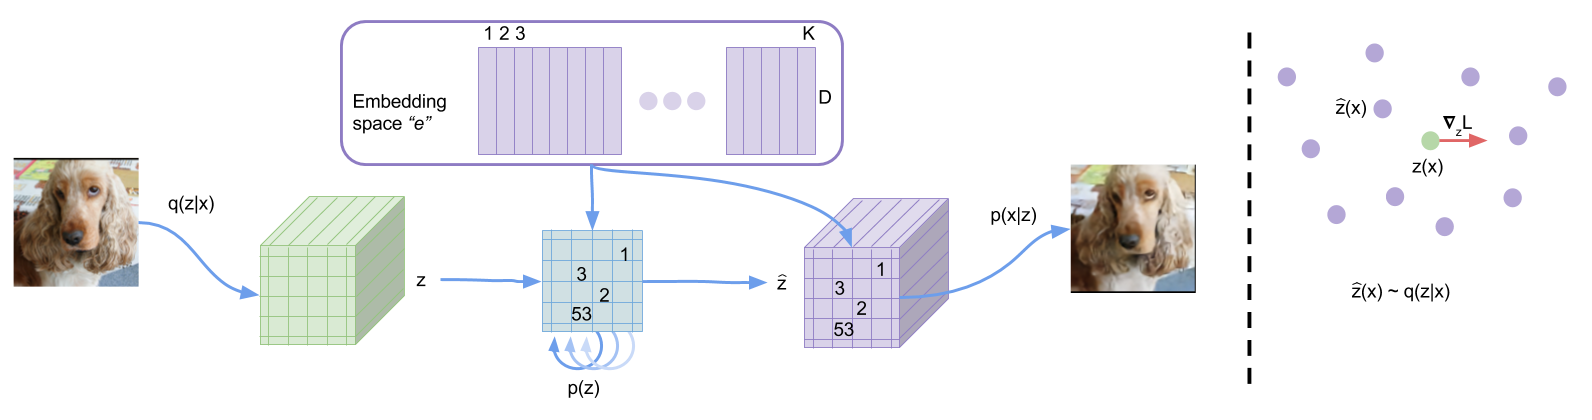
\includegraphics[width=1\linewidth]{figures/chapter02/VQ-VAE.png}
    \caption{Vector Quantised Variational AutoEncoder (VQ-VAE). \newline{}Fuente: Neural Discrete Representation Learning \cite{oord2018neuraldiscreterepresentationlearning}}
    \label{fig:vq-vae}
\end{figure}